%Define sejarah penanggalan,bulan dan tahun
%kelompok 4 D4 TI-2D
%Ayu Permata Sari        1154022
%Librantara Erlangga     1154071
%Martin Luter Zega       1154120
%Putri Aulia Ramadhanie  1154096
%Ryan Hafizh Herdiana    1154067
%Copyright (c) 2017 Copyright Holder All Rights Reserved.


\section{Sejarah penanggalan}
  Penanggalan merupakan salah satu sebuah mahakarya yang bisa ditemukan oleh umat manusia. Manusia mempelajari dan memanfaatkan alam [Matahari,Bulan dan Bintang] untuk menghitung pergantian tanggal,bulan dan juga tahun.
umumnya penanggalan digunakan untuk mengetahui waktu yang telah dilewati oleh umat manusia. Adanya sistem penanggalan ini membuat manusia dapat mengingat seluruh kejadian dan peristiwa yang terjadi di dunia ini.
Menurut artikel dari setyanto berdasarkan benda langit yang digunakan sebagai dasar perhitungan sistem penanggalan dapat dikategorikan menjadi 3 kelompok\cite{setyanto2015kriteria}.

  \subsection{Solar calendar/Kalender Surya}
    Kalender surya menggunakan pergerakan bumi mengelilingi matahari sebagai acuannya.Sistem kalender surya ini biasa digunakan oleh orang-orang eropa. Beberapa contoh kalender yang menggunakan sistem ini yaitu:

    \subsubsection{Julian calendar/Kalender Julian}
      Kalender julian merupakan contoh kalender yang menerapkan sistem surya menurut artikel dari rachmanplanet\cite{rachmanplanet}.Kalender ini telah digunakan bahkan 45 tahun sebelum masehi.
    Awalnya ketika Julius Caesar memimpin pemerintahn romawi terjadi kekacauan  pada perhitungan kalender yang menyebabkan Julis Caesar saat itu mengakhirinya dengan membuat perhitungan kalender sendiri dengan ketentuan:
      1)Satu tahun ditetapkan 565,25 Hari
      2)Tahun biasa, yaitu tiga tahun berturut-turut yang harinya berjumlah 365 Hari
      3)Tahun Kabisat, yaitu tahun keempat ditambah satu hari menjadi 366 Hari.Tambahannya dilakukan pada bulan februari yang jika pada tahun biasa 28 hari pada tahun kabisat ini menjadi 29 hari
      4)Titik permulaan musim semi/bunga ditetapkan pada tanggal 24 Maret
      5)Permulaan tahun ditetapkan pada tanggal 1 Januari (Sebelumnya awal tahun ditetapkan pada tanggal 24 Maret)
    Meskipun kalender julian sudah sangat baik namun ternyata masih terdapat cacat pada kalender tersebut.
    Sebelum orang romawi menggunakan kalender julius caesar, orang romawi sudah menggunakan nama-nama bulan seperti:
    \begin{enumerate}
      \item  Martius     = 31 hari
      \item  Aprilis     = 29 hari
      \item  Majus       = 31 hari
      \item  Junius      = 29 hari
      \item  Quintilis   = 31 hari
      \item  Sextilis    = 29 hari
      \item  September   = 29 hari
      \item  October     = 31 hari
      \item  November    = 29 hari
      \item  Dcember     = 29 hari
      \item  Januarius   = 29 hari
      \item  Februarius  = 28 hari
    \end{enumerate} 

    \subsubsection{Gregorian calendar/Kalender Gregorius}
      Pada tahun 1582 Masehi Paus Gregorius menyaksikan musim semi/bunga pada tanggal 11 maret,bukan lagi pada tanggal 24 maret seperti pada kalender julian.Kemudian paus gregorius memperbaikinya dengan cara:
      1)Musim semi/bunga ditetapkan pada tanggal 21 Maret
      2)Tahun biasa menjadi 365 hari dan tahun kabisat menjadi 566 hari
      Kalender gregorius lebih dikenal dengan nama kalender masehi yang jumlah hari pada setiap bulan dan pentapan awal tahun seperti yang digunakan kalender umumnya saat ini.Kalender masehi dimulai dari tanggal 1 januari
      tahun 1, pukul 00.00.Penamaan bulan pada kalender gregorius yang digunakan hingga sekarang:
      \begin{enumerate}
        \item  January   = 31 hari
        \item  February  = 28/29 hari
        \item  March     = 31 hari
        \item  April     = 30 hari
        \item  May       = 31 hari
        \item  June      = 30 hari
        \item  July      = 31 hari
        \item  August    = 31 hari
        \item  September = 30 hari
        \item  October  = 31 hari
        \item  November = 30 hari
        \item  December = 31 hari
      \end{enumerate}

 \subsection{lunar calendar/Kalender candra}

    \begin{figure}[ht]
    \centerline{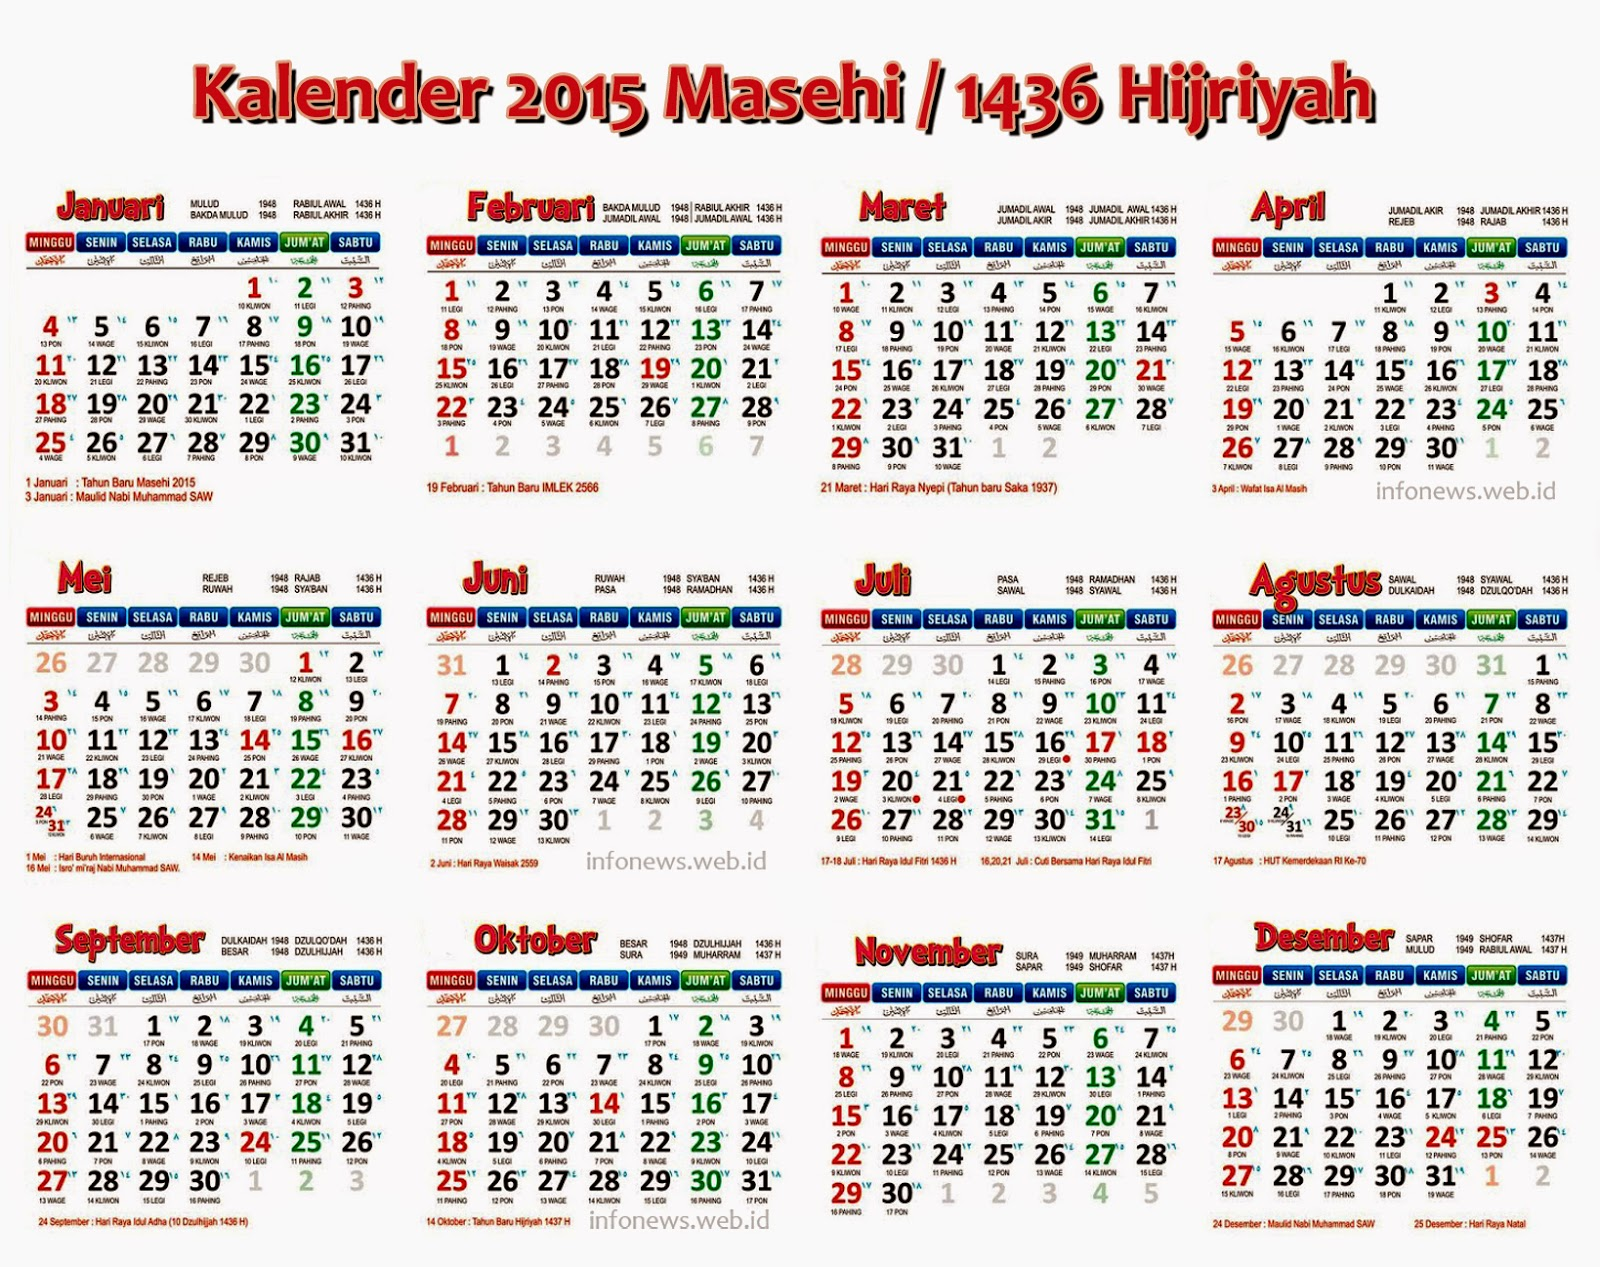
\includegraphics[width=1\textwidth]{figures/Kalender_2015.JPG}}
    \caption{Kalender tahun 2015 Masehi / 1436 Hijriyah.}
    \label{Kalender_2015}
    \end{figure}
    
Pembahasan kelender hijriah terkait dengan sistem penanggalan yang berpedoman pada pergerakan Bulan tampak dari Bumi yaitu ketika Matahari dan Bulan yang berada pada posisi bujur astronomi yang sama. Konjungsi merupakan pergerakan pada posisi Bulan dan Matahari yang terlah disepakati sebagai batas penentuan secara astronomis pada kelender Hijriah.
  Bulan yang berkonjungsi searah dengan Matahari akan tampak gelap pada permukaannya ketika dilihat dari Bumi dengan bentuk cahaya sabit kecil. Bulan baru adalah piringan kecil Bulan yang muncul setelah mengalami satu putaran penuh pada fase Bulan mengelilingi Bumi.
  Kemunculan hilal (bulan baru) merupakan penentuan awal bulan dalam Kelender Hijriah di Indonesia, terkhusus pada bulan Ramadhan, Syawal, dan Zulhijah.Kalender merupakan sistem pengorganisasian waktu yang berfungsi sebagai penanda perhitungan dalam jangka panjang. Kelender hijriah termasuk jenis kelender yang penanggalannya berpatokan pada Bulan ketika mengorbit kepada Bumi.
  Perbedaan antara tahun syamsiah dan tahun kamariah yaitu umur hari dalam satu tahun yang 11 hari juga berbeda dalam penentuan awal perhitungan hari. Penanggalan kamariah memiliki perhitungan yang dimulai sejak terbenamnya Matahari dan berakhir ketika Matahari terbenam pada hari esoknya.
  Sistem penanggalan Islam atau kalender hijriah adalah sistem penanggalan yang memiliki dua belas bulan, dimulai sejak Bulan baru hingga penampakan bulan baru berikutnya berkisar selang waktu antara 29 sampai 30 hari. Revolusi bulan mengililingi bumi memiliki bentuk lintasan yang elips dengan kecepatan tempuh total dalam satu tahun adalah 354 hari 48 menit dan 34 detik.
  Bulan sebagai salah satu komponen penting dalam penanggalan kamariah yakni merupakan satelit tunggal yang dimiliki Bumi. Bulan memiliki 3 pergerakan, diantaranya pergerakan rotasi atau Bulan berputar pada porosnya, revolusi terhadap bumi dan revolusi bersamaan dengan bumi terhadap matahari.

    \subsubsection{Sejarah Kalender Hijriyah}

      Pada saat Sebelum peristiwa haji Wada’ yang dilaksanakan oleh Nabi dan kaum Muslimin, sistem penanggalan masyarakat Arab di Makkah kala itu masih menggunakan konsep penanggalan al-Nasī’. Keberadaan istilah waktu al-Nasī’ tersebut telah mempersulit untuk merunutkan fenomena/peristiwa yang terjadi sebelum haji Wada’\cite{setyanto2015kriteria}.
    Hal ini dikarenakan aturan penggunaan waktu al-Nasī’ tidak berjalan dengan baik. Bangsa Arab dikenal sering memundur dan memajukan kegiatan-kegiatan yang dilakukan pada bulan-bulan Haram sesuai dengan kebutuhannya.4 Hal inilah yang menjadikan penanggalan masyarakat Arab sebelum Haji Wada’ dapat dikatakan tidak konsisten.
    Maksud istilah waktu al-Nasī’ (waktu pengunduran) yaitu diundurnya waktu untuk melaksanakan suatu kegiatan pada waktu tertentu. Salah satunya adalah pengunduran waktu ibadah haji oleh masyarakat Arah ketika itu. Mereka terkadang melaksanakan ibadah haji pada waktunya, terkadang pula pada bulan Muharam, Ṣafar, dan bulan-bulan lainnya di antara dua belas bulan.
    Dampaknya, adalah hal-hal yang mereka yang biasanya dilakukan pada bulan-bulan haram menjadi terabaikan. Hal ini dikarenakan pada saat mereka sedang melaksanakan ibadah haji, mereka bertemu dengan pembunuh ayah mereka, atau bertemu dengan pembunuh sanak saudara mereka, yang menyebabkan mereka membalas dendam pada waktu tersebut.
    Padahal Allah telah menerangkan bahwa melakukan amalan-amalan saleh pada bulan-bulan tersebut merupakan sebesar-besarnya pahala. Sebaliknya, perbuatan zalim yang dilakukan pada saat itu seburuk-buruknya kesalahan, bahkan menambah kekafiran.
    Namun demikian, konsep al-Nasī’ dimaksudkan untuk menyesuaikan fase Bulan dengan perubahan musim yang diakibatkan oleh posisi dan gerak Matahari di Jazirah Arab.Sehingga dapat dikatakan penanggalan masyarakat Arab ketika itu termasuk menggunakan sistem Penanggalan Matahari-Bulan (Kala Surya-Chandra).
    Meski demikian, Nabi Muhammad beserta umat Islam kala itu mengikuti kalender yang sedang berjalan. Sehingga dapat dikatakan seluruh hidup Nabi Muhammad berpuasa dalam sistem penanggalan yang ditetapkan oleh bangsa Quraisy. Nabi tidak membuat sistem penanggalannya sendiri.Turunnya QS.
    al-Taubah [9]: 36-37, yang melarang penggunaan yaum al-Nasi’ (waktu pengunduran) telah mengubah sistem penanggalan masyarakat Arab dari sistem Lunisolar Calendar menjadi sistem Lunar Calender. hal Inilah yang menjadi awal mula atau kelahiran sistem penanggalan Islam yang berbasis pada pergerakan Bulan dalam mengelilingi Bumi.
    Hingga saat ini belum diketahui dengan baik bagaimana praktek penanggalan Islam pada zaman sahabat. Namun, diyakini penanggalan Islam pada masa itu didasarkan pada kesaksian ru’yat al-hilāl. Adapun proses bagaimana praktek penanggalan Hijriyah sejak berubahnya sistem penanggalan tersebut pada dasarnya dapat ditelusuri melalui sejarah, sebagaimana yang telah dilakukan oleh Saleh al-Saab dari King Abdul’aziz City for Science and Technology (KACST), Riyadh.
    Praktek penanggalan Islam kemudian disempurnakan melalui konsep penanggalan yang dirumuskan pada zaman Umar bin Khaṭṭab. Melalui sidang para sahabat rasulullah, ditetapkanlah perhitungan tahun dalam penanggalan kekhalifahan, dimulai sejak hijrahnya Nabi Muhammad dari Mekkah ke Madinah.
    Penetapan tahun hijrahnya Nabi sebagai tahun pertama tersebut merupakan usulan dari Sahabat ‘Ali bin Abī Ṭālib.11 Oleh karena itu, penanggalan kekhalifahan Islam dikenal sebagai penanggalan Hijriyah, dengan bulan Muharam sebagai bulan pertama dalam penanggalan tersebut. Hal tersebutlah yang telah umum berlaku di masyarakat Arab ketika itu.
    Sama halnya dengan penanggalan Masehi yang digunakan saat ini, penanggalan Hijriyah pun pada zaman sahabat ditetapkan berdasarkan perhitungan matematis. Jumlah hari yang digunakan senantiasa tetap setiap bulannya. Meskipun demikian, hal-hal yang terkait dengan pelaksanaan ibadah kaum Muslimin kala itu tetap mengikuti ketentuan yang telah diajarkan oleh Nabi Muhammad.
    Oleh karenanya, penanggalan pada kalender Hijriyah yang telah ditetapkan merupakan penanggalan Administrasi Negara.Seiring dengan perkembangan pemahaman dan pengetahuan, saat ini fungsi penanggalan Hijriyah sebagai penanggalan sosial menjadi satu kesatuan dengan fungsinya sebagai penanggalan ibadah. Hal inilah yang dilihat secara subyektif sebagai kisruh sistem penanggalan Hijriyah.
    Maka dari itu, untuk mengurai permasalahan pada tahap awal adalah dengan melepaskan fungsi ibadah dari sistem penanggalan Hijriyah.Namun, aturan ibadah tetap menjadi acuan dalam penyusunan kalender Hijriyah, sebagaimana yang telah dipraktekkan oleh sahabat. Dalam beribadah terdapat kesepakatan pada proses pencapaian kesatuan dalam beribadah yaitu dapat diawali dengan menyepakati penggunaan kalender tunggal yang digunakan bersama, sedangkan pelaksanaan ibadah dikembalikan kepada masing-masing.Berikut adalah nama bulan dan hari pada kalender hijriyah berdasarkan pada hisab urfi:
    \begin{enumerate}
        \item Muharram      = 30 hari
        \item Shafar        = 29 hari
        \item Rabiul Awwal  = 30 hari
        \item Rabiul Akhir  = 29 hari
        \item Jumadil Awwal = 30 hari
        \item Jumadil Akhir = 29 hari
        \item Rajab         = 30 hari
        \item Shaban        = 29 hari
        \item Ramadhan      = 30 hari
        \item Syawal        = 29 hari
        \item Dzulka'idah   = 30 hari
        \item Dzhulhijjah   = 29/30 hari
    \end{enumerate}

  \subsection{lunisolar calendar/kalender suryacandra}

      Menurut wicaksono dalam artikelnya Lunisolar kalender merupakan sistem kalender candra yang disesuaikan dengan matahari \cite{wicaksono2008ta}.Karena kalender candra dalam 1 tahun mempunyai 11 hari lebih cepat dari kalender surya, maka dalam kalender suryacandra memiliki bulan interkalasi(bulan tambahan/bulan ke -13)setiap 3 tahun, agar kembali seusai dengan perjalanan matahari.
    beberapa contoh kalender yang mengacu pada sistem suryacandra adalah kalender imlek/cina,saka dan budhha. Semua kalender tersebut tidak ada yang sempurna ,karena jumlah hari dalam satu tahun itu tidak bulat,dan untuk memperkecil error itu maka dibuat kesepakatan sehari lebih panjang atau terdapat bulan tambahan dalam kalender cina pada tahun kabisat\cite{wicaksono2008ta}.
    Pada kalender surya, pergantian hari terjadi tengah malam dan awal setiap bulan (tanggal 1) yang tidak tergantung pada posisi bulan dan pada kalender candra dan suryacandra pergantian hari terjadi ketika matahari terbenam dan awal setiap bulan adalah saat konjungsi(imlek,sakka,budhha) atau dalam hijriyah saat munculnya hilal.
